\documentclass[a4paper]{article}

\usepackage{fullpage} % Package to use full page
\usepackage{parskip} % Package to tweak paragraph skipping
\usepackage{tikz} % Package for drawing
\usepackage{amsmath}
\usepackage{hyperref}
\usepackage{graphicx}

\title{Programming Project: Restricted Boltzmann Machine}
\author{Christoph Kirchner\\Mario Rose\\Nga Pham}
\date{21/2/2018}

\begin{document}

\maketitle
\section{Introduction}
For this assignment we implemented a generic RBM over binary random variables, trained and tested MNIST example with different settings in order to achieve better result.\\
Please note, that in the following results, if not stated otherwise, we used following default settings:
\begin{itemize}
    \item Maximum epochs: 1.000
    \item Sample data size of 10.000
    \item Learning rate: 0.1
    \item Number of random instances: 1.000
    \item Number of repetition in Gibbs sampling techniques: 5
    \item Number of samples in Markov chains: 10
    \item Number of visible units: 784 (one for every pixel in the training images)
    \item Number of hidden units: 1000
\end{itemize}


\section{Implement a generic RBM}
To implement our generic RBM over binary random variables, we followed the theory of the lecture slides:
\begin{enumerate}
    \item Initial class RBM with weights for visible, hidden and bias unit.
    \item Create training algorithm. We used Persistent Contrastive Divergence (PCD).
    \item Handle data: We used the original MNIST test set for training and binarized it. The code snippet was from the assignment description.
\end{enumerate}
\newpage
\section{Train the machine on MNIST data and draw random images}
Best results with GibbsSampling, 20000 epochs, 1000 hidden units and Chain length of 20: \\
(The Random Number Generator took 2 times 8)\\
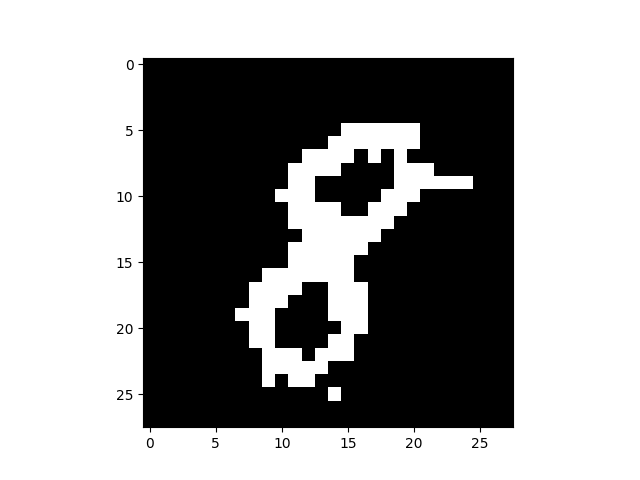
\includegraphics[width=0.5\textwidth]{Figure_1-19.png}
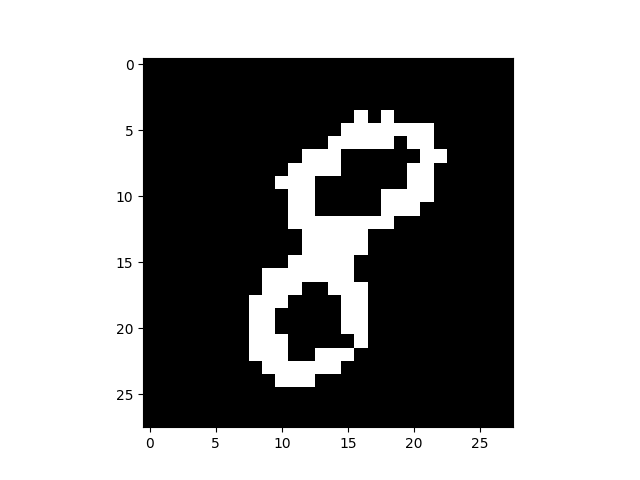
\includegraphics[width=0.5\textwidth]{Figure_1-39.png}
\includegraphics[width=0.5\textwidth]{six.png}
\newline
10 randomly drawn images for digit 8 and 6:\\
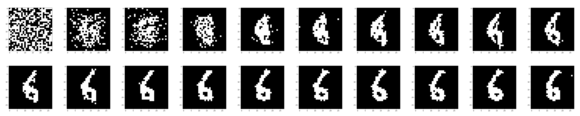
\includegraphics[width=0.75\textwidth]{6_chain_20.png}\\
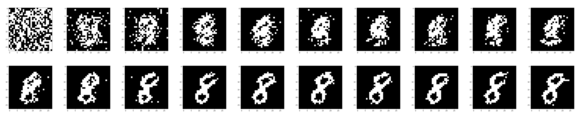
\includegraphics[width=0.75\textwidth]{8_chain_20.png}
\newpage
\section{Explore the number of hidden units}
Gibbs Sampling, 5000 epochs, Chain length 20\\\\
500 hidden units:\\
\includegraphics[width=0.5\textwidth]{500_hidden_nodes.png}\\
784 hidden units:\\
\includegraphics[width=0.5\textwidth]{784_hidden_nodes.png}\\
1000 hidden units:\\
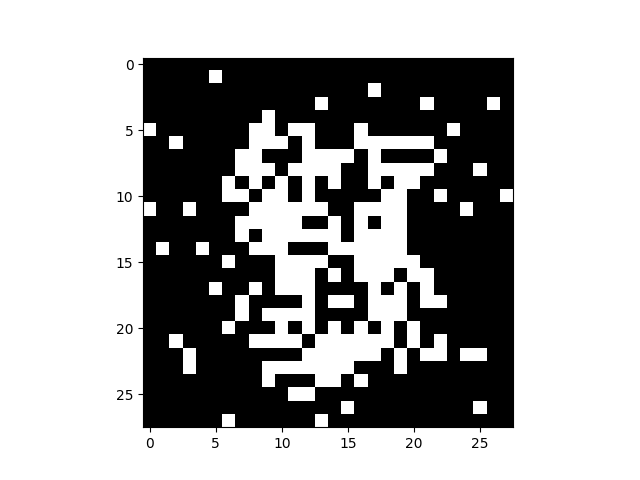
\includegraphics[width=0.5\textwidth]{Figure_1-1.png}
\section{Explore different number of Markov chains}
GibbsSampling, 20000 epochs, 1000 hidden units\\
\\
Chain Length of 5:\\
\includegraphics[width=0.5\textwidth]{8_chainLength5.png}
\includegraphics[width=0.5\textwidth]{6_chainLength5.png}
Chain Length of 10:\\
\includegraphics[width=0.5\textwidth]{8_chainLength10.png}
\includegraphics[width=0.5\textwidth]{6_chainLength10.png}
Chain Length of 15:\\
\includegraphics[width=0.5\textwidth]{8_chainLength15.png}
\includegraphics[width=0.5\textwidth]{6_chainLength15.png}
\newpage
Chain Length of 20:\\
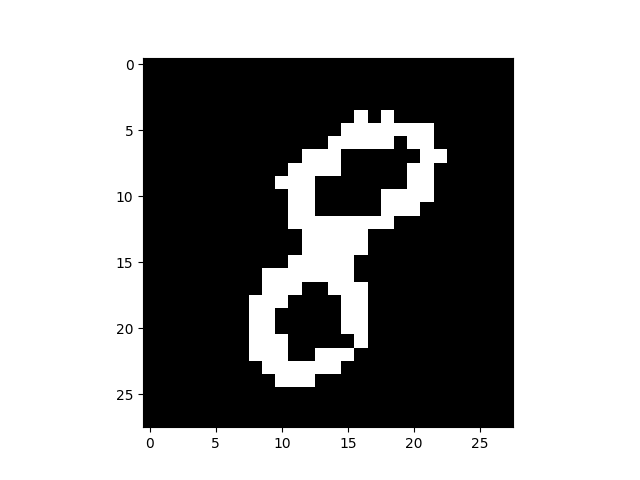
\includegraphics[width=0.5\textwidth]{Figure_1-39.png}
\includegraphics[width=0.5\textwidth]{six.png}\\
These results show that the higher the number of Markov Chains, the better the result.\\
But the results with a length of 15 look almost as good as the results with 20, which leads to the conclusion that there will probably be a point where increasing the number of Markov Chains does not increase the quality of the generated image any more.
\section{Gibbs Sampling}
Without Gibbs Sampling, 30000 epochs:\\
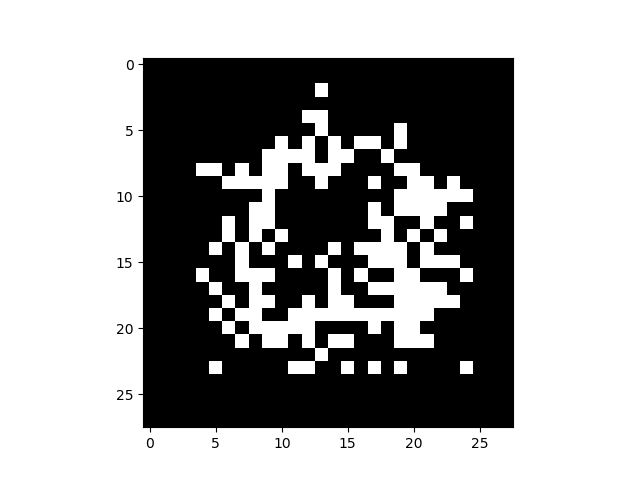
\includegraphics[width=0.5\textwidth]{Figure_30000_2-10.png}\\
With Gibbs Sampling, 20000 epochs:\\
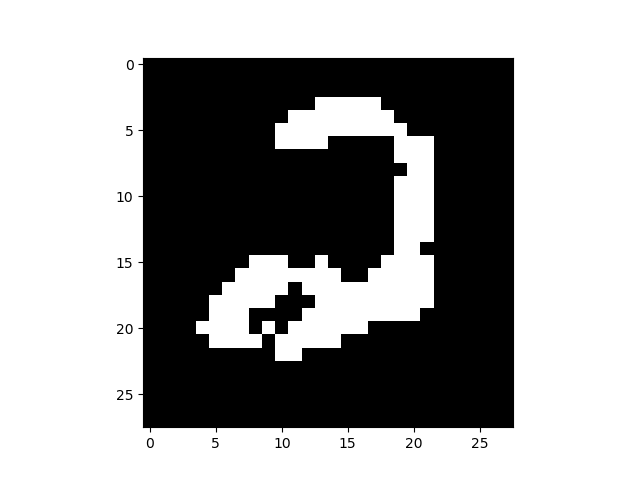
\includegraphics[width=0.5\textwidth]{Figure_1-9.png}\\
It is obviously that using Gibbs Sampling gave better results.
\section{Explore Adaptive Learning Rate}
We observed if adjustment in learning rate impacts the performance of the trained RBM. We tested the case in which the learning rate was increased and decreased gradually by multiplying the original with (1 + $\epsilon$) and (1 - $\epsilon$), respectively. $\epsilon$ is a constant, in this case we used learning rate = 0.01 and $\epsilon$ = 0.001. 
\begin{verbatim}
    if (learning_rate_decay):
        learning_rate = (1 - epsilon) * learning_rate
\end{verbatim}
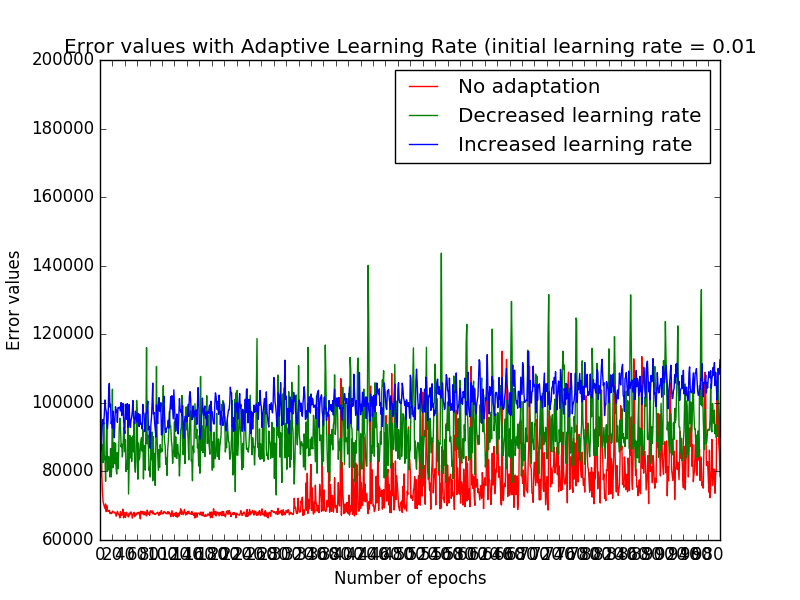
\includegraphics[width=0.6\textwidth]{plot_adaptiveLr.png}\\
As stated in the above figure, best result can be achieved with original learning rate, then the decreased learning rate. However, they lead to more fluctuate error values curve than the case of increased learning rate.\\
Reference: G. Hinton, \textit{“A Practical Guide to Training Restricted Boltzmann Machines”}. Neural Networks: Tricks of the Trade, 2nd edition, pp. 599–619, 2012
\section{Explore the length of the burn-in phase in Gibbs sampling}
We explored the impact of burn-in phase by drop out the first few states of the Markov chain. The cases when first 100 and 1000 states are thrown away are tested. 
\begin{verbatim}
    if (burn_in_drop):
        for j in range(1, num_drop):
            hidden_states[:j] = 0  # Start dropping out first 100 states in Gibbs sampling
\end{verbatim}
The plot below compared two results:

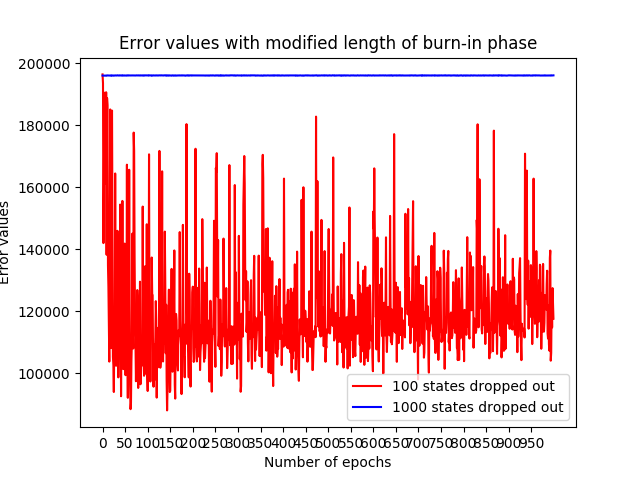
\includegraphics[width=0.6\textwidth]{plot_burnIn.png}\\
It is obvious that with 100 states dropped out, the result was much better, however, produced significantly fluctuate curve. Error values in case of 1000 states is stable, around 200.000 for each epochs. This may lead to a prediction that there will be a point that increasing the states will not decrease the error values anymore.
\end{document}